\documentclass[a4paper,11pt,openright,oneside]{report}
\usepackage[utf8]{inputenc}
\usepackage[margin=3cm]{geometry}
\usepackage[T1]{fontenc}
\usepackage[portuguese]{babel}
\usepackage{graphicx}
%\usepackage[backend=biber,style=ieee]{biblatex}
\usepackage{csquotes}
\usepackage{blindtext}
\usepackage[printonlyused]{acronym}
\usepackage{hyperref}
\usepackage{minted}
\usepackage[titletoc,title]{appendix}
\usepackage{caption}
\usepackage{subcaption}
\newcommand{\RNum}[1]{\uppercase\expandafter{\romannumeral #1\relax}}

\begin{document}

\title{\textbf{Comando Infra-Vermelhos no Controlo de LEDs}\\[1cm]\textsc{\small {Departamento de Electrónica, Telecomunicações e Informática} \\ \large {UNIVERSIDADE DE AVEIRO}}}
\author{Sandra Moreira 76471, Ricardo Jesus 76613\\simoreira@ua.pt, ricardojesus@ua.pt}
\date{1 de Junho de 2015}
\maketitle
\pagenumbering{arabic}

\chapter{Infra-Vermelhos no Controlo de LEDs}

\section{Introdução}
\label{sec:introdução}

No âmbito da unidade curricular de Laboratórios de Sistemas Digitais, foi proposta a elaboração de um mini-projeto relativo aos conteúdos abordados ao longo do semestre. Neste sentido, foi desenvolvido um módulo de infra-vermelhos que permite controlar várias componentes do KIT DE2-115 da Terasic através do comando que acompanha este, de acordo com o tema apresentado e escolhido no guião de propostas. Fundamentalmente, a partir do comando deverá ser possível controlar o número de LEDs verdes acessos do KIT, em função da tecla premida, bem como a sua intensidade.

\section{Arquitetura do Sistema}
\label{sec:arquitetura}



\section{Implementação}
\label{sec:implementação}



\section{Validação de Resultados}
\label{sec:validação}



\section{Conclusão}
\label{sec:conclusão}

\begin{figure}[ht]
\center
\fbox{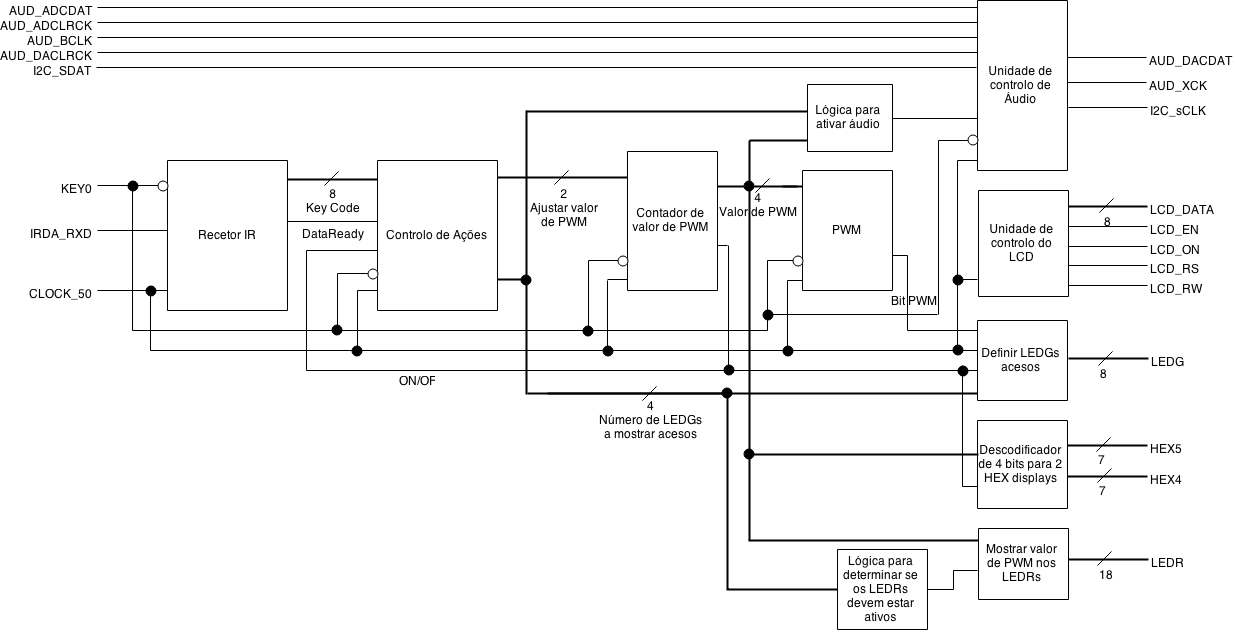
\includegraphics[height=7cm]{img/ir_leds0}}
\caption{Funções suportadas do comando utilizado}
\label{fig:ir_leds0}
\end{figure}

\maketitle
\nocite{*}

\end{document}
